  
\documentclass[11pt,a4paper,professionalfonts]{article}


\usepackage{amssymb,amsmath}
\usepackage{amsthm}
\usepackage{graphics}
\usepackage{scalefnt}
\usepackage{graphicx}
\usepackage[spanish,english, activeacute]{babel}
\usepackage[utf8x]{inputenc}
\usepackage{ucs}
\usepackage{listings}
\usepackage{color}
\usepackage{verbatim}
\usepackage{fancyvrb}
\usepackage{relsize}
\usepackage[below]{placeins}
\usepackage[vlined,ruled,linesnumbered,commentsnumbered]{algorithm2e}        
% used for pseudocode
\usepackage{url}
\usepackage[margin=3cm,top=3.5cm,bottom=3.5cm]{geometry}

\usepackage{minted}
\usepackage{xcolor}

\definecolor{mintedbackground}{rgb}{0.97,0.97,0.97}

\newminted{java}{
baselinestretch=0.85,
bgcolor=mintedbackground,
fontfamily=tt,
fontsize=\footnotesize,
xleftmargin=0pt,
linenos=false,
numberblanklines=true,
numbersep=12pt,
numbersep=5pt,
gobble=0,
frame=none,
framerule=0.4pt,
framesep=2mm,
funcnamehighlighting=true,
tabsize=4,
obeytabs=false,
mathescape=false
samepage=false, %with this setting you can force the list to appear on the same page
showspaces=false,
showtabs =false,
texcl=false,
} 

\newmintedfile[archivoLargo]{java}{
fontfamily=tt,
baselinestretch=1,
fontsize=\relsize{+0},
xleftmargin=130pt,
linenos=true,
numberblanklines=true,
numbersep=12pt,
numbersep=5pt,
gobble=0,
frame=none,
framerule=0.4pt,
framesep=2mm,
funcnamehighlighting=true,
tabsize=4,
obeytabs=false,
mathescape=false,
samepage=false, %with this setting you can force the list to appear on the same page
showspaces=false,
showtabs =false,
texcl=false,
}


\def\lstlistingname{Listado}

\graphicspath{{Images/}}

\author{Metodología de la programación, doble grado, 2013-2014}
\title{\vspace{-3cm}\begin{center} \line(1,0){370} \\\vspace{0.5cm} \end{center}
Uso de la herramienta VALGRIND}
\date{}


\newcommand{\bX}{\mathbf{X}}
\newcommand{\bx}{\mathbf{x}}
\newcommand{\bY}{\mathbf{Y}}
\newcommand{\by}{\mathbf{y}}
\newcommand{\bZ}{\mathbf{Z}}
\newcommand{\bz}{\mathbf{z}}
\newcommand{\bE}{\mathbf{E}}
\newcommand{\be}{\mathbf{e}}
\newcommand{\domi}{\Omega_{X_i}}
\newcommand{\domb}{\Omega_{X_b}}
\newcommand{\dom}{\Omega_{\bX}}
\newcommand{\R}{\ensuremath{\mathbb{R}}}
\newcommand{\cT}{\mathcal{T}}
\newcommand{\cR}{\mathcal{RT}}
\newcommand{\indx}{ind(\ensuremath{\mathbf{x})}}
\newcommand{\indxr}{ind_r(\ensuremath{\mathbf{x})}}
\newcommand{\indxl}{ind_l(\ensuremath{\mathbf{x})}}
\newcommand{\indxbr}{ind_{br}(\ensuremath{\mathbf{x})}}


\begin{document}

\renewcommand{\contentsname}{Contenido:}

\maketitle
\vspace{-1.5cm}
\begin{center} \line(1,0){370} \end{center}
\vspace{0.5cm}

\tableofcontents
\vspace{-0.3cm}
\begin{center} \line(1,0){370} \end{center}
\vspace{0.5cm}

\section{¿Qué es?}

\textbf{Valgrind} es una plataforma de análisis del código. Contiene un conjunto
de herramientas que permiten detectar problemas de memoria y también obtener
datos detallados de la forma de funcionamiento (rendimiento) de un programa.
Es una herramienta de libre distribución que puede obtenerse en: 
\url{valgrind.org}. ¡No está disponible para Windows! Algunas de las herramientas 
que incorpora son:

\begin{itemize}
\item \textbf{memcheck}: detecta errores en el uso de la memoria dinámica
\item \textbf{cachegrind}: permite mejorar la rapidez de ejecución del código
\item \textbf{callgrind}: da información sobre las llamadas a métodos producidas
por el código en ejecución
\item \textbf{massif}: ayuda a reducir la cantidad de memoria usada por el programa.
\end{itemize}


Nosotros trabajaremos básicamente con la opción de chequeo de problemas de memoria. Esta
es la herra\-mienta de uso por defecto. El uso de las demás se indica mediante la opción
\textbf{tool}. Por ejemplo, para obtener información sobre las llamadas a 
funciones y métodos mediante \textbf{callgrind} haríamos:


\begin{verbatim}
             valgrind --tool=callgrind .........
\end{verbatim}


Quizás la herramienta más necesaria sea la de chequeo de memoria (por eso es
la opción por defecto). La herramienta \textbf{memchek} presenta varias
opciones de uso (se consideran aquí únicamente las más habituales):

\begin{itemize}
\item \textbf{leak-check}: indica al programa que muestre las fugas de memoria
al finalizar la ejecución del programa. Los posibles valores para este argumento
son \textbf{no}, \textbf{summary}, \textbf{yes} y \textbf{full}

\item \textbf{undef-value-errors}: controla si se examinan los errores debidos a
variables no inicializadas (sus posibles valores son \textbf{no} y \textbf{yes},
siendo este último el valor por defecto)

\item \textbf{track-origins}: indica si se controla el origen de los valores no
inicializados (con \textbf{no} y \textbf{yes} como posibles valores, siendo el
primero el valor por defecto). El valor de este argumento debe estar en concordancia
con el del argumento anterior (no tiene sentido indicar que no se desea información
sobre valores no inicializados e indicar aquí que se controle el origen de los
mismos)
\end{itemize}

Una forma habitual de lanzar la ejecución de esta herramienta es la siguiente 
(observad que el nombre del programa y sus posibles argumentos van al final
de la línea):

\begin{verbatim}
              valgrind --leak-check=full --track-origins=yes ./programa
\end{verbatim}

Esta forma de ejecución ofrece información detallada sobre los posibles
problemas en el uso de la memoria dinámica requerida por el programa. Iremos
considerando algunos ejemplos para ver la salida obtenida en varios escenarios. 
Es importante tener en cuenta que es preciso compilar los programas
con la opción \textbf{-g} para que se incluya información de depuración en
el ejecutable. 

\section{Chequeo de memoria: algunos problemas frecuentes}

Se consideran a continuación algunos ejemplos de código con problemas usuales
en código con gestión dinámica de memoria. Se analizan para ver qué mensajes
de aviso nos muestra esta herramienta en cada caso.

\subsection{Uso de memoria no inicializada}

Imaginemos que el siguiente código se encuentra en un archivo llamado 
\textbf{ejemplo1.cpp}.

\archivoLargo{./codigo/ejemplo1.cpp}

Compilamos mediante la sentencia:

\begin{verbatim}
              g++ -g -o ejemplo1 ejemplo1.cpp
\end{verbatim}

Si ejecutamos ahora \textbf{valgrind} como hemos visto antes:

\begin{verbatim}
              valgrind --leak-check=full --track-origins=yes ./ejemplo1
\end{verbatim}

\noindent se obtiene un informa bastante detallado de la forma en que el programa usa
la memoria dinámica. Parte del informe generado es:

\vspace{0.4cm}
\begin{javacode}
full --track-origins=yes ./ejemplo1
==13420== Memcheck, a memory error detector
==13420== Copyright (C) 2002-2011, and GNU GPL'd, by Julian Seward et al.
==13420== Using Valgrind-3.7.0 and LibVEX; rerun with -h for copyright info
==13420== Command: ./ejemplo1
==13420== 
==13420== Conditional jump or move depends on uninitialised value(s)
==13420==    at 0x4EC4F16: std::ostreambuf_iterator<char, std::char_traits<char> > std::num_put<char, std::ostreambuf_iterator<char, std::char_traits<char> > >::_M_insert_int<long>(std::ostreambuf_iterator<char, std::char_traits<char> >, std::ios_base&, char, long) const (in /usr/lib/x86_64-linux-gnu/libstdc++.so.6.0.17)
==13420==    by 0x4EC514C: std::num_put<char, std::ostreambuf_iterator<char, std::char_traits<char> > >::do_put(std::ostreambuf_iterator<char, std::char_traits<char> >, std::ios_base&, char, long) const (in /usr/lib/x86_64-linux-gnu/libstdc++.so.6.0.17)
==13420==    by 0x4EC8015: std::ostream& std::ostream::_M_insert<long>(long) (in /usr/lib/x86_64-linux-gnu/libstdc++.so.6.0.17)
==13420==    by 0x400922: main (ejemplo1.cpp:6)
==13420==  Uninitialised value was created by a stack allocation
==13420==    at 0x40090C: main (ejemplo1.cpp:4)
==13420== 
==13420== Use of uninitialised value of size 8
==13420==    at 0x4EBA343: ??? (in /usr/lib/x86_64-linux-gnu/libstdc++.so.6.0.17)
==13420==    by 0x4EC4F37: std::ostreambuf_iterator<char, std::char_traits<char> > std::num_put<char, std::ostreamvalgrindbuf_iterator<char, std::char_traits<char> > >::_M_insert_int<long>(std::ostreambuf_iterator<char, std::char_traits<char> >, std::ios_base&, char, long) const (in /usr/lib/x86_64-linux-gnu/libstdc++.so.6.0.17)
...................................................
\end{javacode}
\vspace{0.4cm}

Si nos fijamos en los mensajes que aparecen en el informe anterior 
(\textbf{Conditional jump or move depends on uninitialised values} - 
\textbf{use of uninitialised value of size 8}) se alude a que los valores 
del array no han sido inicializados y que se pretende usar el contenido de 
una posición no inicializada. Si arreglamos el código de forma conveniente y
ejecutamos de nuevo, veremos que desaparecen los mensajes de error:

\archivoLargo{./codigo/ejemplo1-ok.cpp}
valgrind
El informe de que todo ha ido bien es el siguiente:

\vspace{0.4cm}
\begin{javacode}
==13504== Memcheck, a memory error detector
==13504== Copyright (C) 2002-2011, and GNU GPL'd, by Julian Seward et al.
==13504== Using Valgrind-3.7.0 and LibVEX; rerun with -h for copyright info
==13504== Command: ./ejemplo1-ok
==13504== 
==13504== 
==13504== HEAP SUMMARY:
==13504==     in use at exit: 0 bytes in 0 blocks
==13504==   total heap usage: 0 allocs, 0 frees, 0 bytes allocated
==13504== 
==13504== All heap blocks were freed -- no leaks are possible
==13504== 
==13504== For counts of detected and suppressed errors, rerun with: -v
==13504== ERROR SUMMARY: 0 errors from 0 contexts (suppressed: 2 from 2)
\end{javacode}
\vspace{0.4cm}

No debemos hacer caso a la indicación final de usar la opción \textbf{-v} (modo
\textbf{verbose}). Si se usa se generaría una salida mucho más extensa que nos informa
de errores de la propia librería de \textbf{valgrind} o de las librerías aportadas
por C++ (lo que no nos interesa, ya que no tenemos posibilidad de reparar sus
problemas).

\subsection{Lectura y/o escritura en memoria liberada}

Supongamos ahora que el código analizado es el siguiente:

\archivoLargo{./codigo/usoMemoriaLiberada/usoMemoriaLiberada.cpp}

El análisis de este código ofrece el siguiente informe valgrind

\vspace{0.4cm}
\begin{javacode}
==2408== Memcheck, a memory errvalgrindor detector
==2408== Copyright (C) 2002-2012, and GNU GPL'd, by Julian Seward et al.
==2408== Using Valgrind-3.8.1 and LibVEX; rerun with -h for copyright info
==2408== Command: ./usoMemoriaLiberada
==2408== 
==2408== Invalid read of size 1
==2408==    at 0x4008E2: main (usoMemoriaLiberada.cpp:24)
==2408==  Address 0x5a1a040 is 0 bytes inside a block of size 1 free'd
==2408==    at 0x4C2BADC: operator delete(void*) (in /usr/lib/valgrind/vgpreload_memcheck-amd64-linux.so)
==2408==    by 0x4008DD: main (usoMemoriaLiberada.cpp:21)
==2408== 
==2408== 
==2408== HEAP SUMMARY:
==2408==     in use at exit: 0 bytes in 0 blocks
==2408==   total heap usage: 1 allocs, 1 frees, 1 bytes allocated
==2408== 
==2408== All heap blocks were freed -- no leaks are possible
==2408== 
==2408== For counts of detected and suppressed errors, rerun with: -v
==2408== ERROR SUMMARY: 1 errors from 1 contexts (suppressed: 2 from 2)
\end{javacode}
\vspace{0.4cm}

El informe indica explícitamente la línea del código en que se
produce el error (línea 21): lectura inválida (sobre memoria ya
liberada). En esta línea se muestra que se ha hecho la liberación
sobre el puntero \textbf{p}.


\subsection{Sobrepasar los límites de un array en operación de lectura}

Veremos ahora el mensaje obtenido cuando se sobrepasan los límites de un
array:

\archivoLargo{./codigo/ejemplo2.cpp}


Entre los mensajes de error aparece ahora el siguiente texto (parte del informe
completo generado):

\vspace{0.4cm}
\begin{javacode}
==4474== Memcheck, a memory error detector
==4474== Copyright (C) 2002-2012, and GNU GPL'd, by Julian Seward et al.
==4474== Using Valgrind-3.8.1 and LibVEX; rerun with -h for copyright info
==4474== Command: ./ejemplo2
==4474== Parent PID: 1529
==4474== 
==4474== Invalid read of size 4
==4474==    at 0x40088B: main (ejemplo2.cpp:6)
==4474==  Address 0x5a1a068 is 20 bytes after a block of size 20 alloc'd
==4474==    at 0x4C2AFE7: operator new[](unsigned long) (in /usr/lib/valgrind/vgpreload_memcheck-amd64-linux.so)
==4474==    by 0x40087E: main (ejemplo2.cpp:5)
==4474== 
==4474== 
==4474== HEAP SUMMARY:
==4474==     in use at exit: 20 bytes in 1 blocks
==4474==   total heap usage: 1 allocs, 0 frees, 20 bytes allocated
==4474== 
==4474== 20 bytes in 1 blocks are definitely lost in loss record 1 of 1
==4474==    at 0x4C2AFE7: operator new[](unsigned long) (in /usr/lib/valgrind/vgpreload_memcheck-amd64-linux.so)
==4474==    by 0x40087E: main (ejemplo2.cpp:5)
==4474== 
==4474== LEAK SUMMARY:
==4474==    definitely lost: 20 bytes in 1 blocks
==4474==    indirectly lost: 0 bytes in 0 blocks
==4474==      possibly lost: 0 bytes in 0 blocks
==4474==    still reachable: 0 bytes in 0 blocks
==4474==         suppressed: 0 bytes in 0 blocks
==4474== 
==4474== For counts of detected and suppressed errors, rerun with: -v
==4474== ERROR SUMMARY: 2 errors from 2 contexts (suppressed: 2 from 2)
\end{javacode}
\vspace{0.4cm}

Observad el error: (\textbf{Invalid read of size 4} ocurrido en relación
al espacio de memoria reservado en la línea 5). 

\subsection{Sobrepasar los límites de un array en operación de escritura}

También es frecuente exceder los límites del array para escribir en una posición 
que ya no le pertenece (alta probabilidad de generación de \textbf{core}):

\archivoLargo{./codigo/ejemplo3.cpp}


Además del problema mencionado con anterioridad, en este programa no se libera el 
espacio reservado al finalizar. La información ofrecida por \textbf{valgrind} 
ayudará a solucionar todos los problemas mencionados:

\vspace{0.4cm}
\begin{javacode}
==14144== Memcheck, a memory error detector
==14144== Copyright (C) 2002-2011, and GNU GPL'd, by Julian Seward et al.
==14144== Using Valgrind-3.7.0 and LibVEX; rerun with -h for copyright info
==14144== Command: ./ejemplo3
==14144== 
==14144== Invalid write of size 4
==14144==    at 0x400732: main (ejemplo3.cpp:7)
==14144==  Address 0x5a06054 is 0 bytes after a block of size 20 alloc'd
==14144==    at 0x4C2AAA4: operator new[](unsigned long) (in /usr/lib/valgrind/vgpreload_memcheck-amd64-linux.so)
==14144==    by 0x40070D: main (ejemplo3.cpp:5)
==14144== 
==14144== 
==14144== HEAP SUMMARY:
==14144==     in use at exit: 20 bytes in 1 blocks
==14144==   total heap usage: 1 allocs, 0 frees, 20 bytes allocated
==14144== 
==14144== 20 bytes in 1 blocks are definitely lost in loss record 1 of 1
==14144==    at 0x4C2AAA4: operator new[](unsigned long) (in /usr/lib/valgrind/vgpreload_memcheck-amd64-linux.so)
==14144==    by 0x40070D: main (ejemplo3.cpp:5)
==14144== 
==14144== LEAK SUMMARY:
==14144==    definitely lost: 20 bytes in 1 blocks
==14144==    indirectly lost: 0 bytes in 0 blocks
==14144==      possibly lost: 0 bytes in 0 blocks
==14144==    still reachable: 0 bytes in 0 blocks
==14144==         suppressed: 0 bytes in 0 blocks
==14144== 
==14144== For counts of detected and suppressed errors, rerun with: -v
==14144== ERROR SUMMARY: 2 errors from 2 contexts (suppressed: 2 from 2)
\end{javacode}
\vspace{0.4cm}


Observad los dos mensajes de error indicados: escritura inválida de tamaño 4
(tamaño asociado al entero) y en el resumen de memoria usada (leak summary) se 
indica que hay memoria perdida (20 bytes formando parte de un bloque: 
5 $\times$ 4 bytes). Con esta información es fácil arreglar estos problemas:

\archivoLargo{./codigo/ejemplo4.cpp}


De esta forma desaparecen todos los mensajes de error previos:

\vspace{0.4cm}
\begin{javacode}
==14218== Memcheck, a memory error detector
==14218== Copyright (C) 2002-2011, and GNU GPL'd, by Julian Seward et al.
==14218== Using Valgrind-3.7.0 and LibVEX; rerun with -h for copyright info
==14218== Command: ./ejemplo4
==14218== 
==14218== 
==14218== HEAP SUMMARY:
==14218==     in use at exit: 0 bytes in 0 blocks
==14218==   total heap usage: 1 allocs, 1 frees, 20 bytes allocated
==14218== 
==14218== All heap blocks were freed -- no leaks are possible
==14218== 
==14218== For counts of detected and suppressed errors, rerun with: -v
==14218== ERROR SUMMARY: 0 errors from 0 contexts (suppressed: 2 from 2)
\end{javacode}
\vspace{0.4cm}

\subsection{Problemas con delete sobre arrays}

Otro problema habitual al liberar el espacio de memoria usado por un
array suele consistir en olvidar el uso de los corchetes. Esto genera
un problema de uso de memoria, ya que no se indica que debe eliminarse
un array. El código y los mensajes correspondientes de \textbf{valgrind} 
aparecen a continuación:

\archivoLargo{./codigo/ejemplo5.cpp} 

\vspace{0.4cm}
\begin{javacode}
==14364== Memcheck, a memory error detector
==14364== Copyright (C) 2002-2011, and GNU GPL'd, by Julian Seward et al.
==14364== Using Valgrind-3.7.0 and LibVEX; rerun with -h for copyright info
==14364== Command: ./ejemplo5
==14364== 
==14364== Mismatched free() / delete / delete []
==14364==    at 0x4C2A44B: operator delete(void*) (in /usr/lib/valgrind/vgpreload_memcheck-amd64-linux.so)
==14364==    by 0x40078E: main (ejemplo5.cpp:9)
==14364==  Address 0x5a06040 is 0 bytes inside a block of size 20 alloc'd
==14364==    at 0x4C2AAA4: operator new[](unsigned long) (in /usr/lib/valgrind/vgpreload_memcheck-amd64-linux.so)
==14364==    by 0x40074D: main (ejemplo5.cpp:5)
==14364== 
==14364== 
==14364== HEAP SUMMARY:
==14364==     in use at exit: 0 bytes in 0 blocks
==14364==   total heap usage: 1 allocs, 1 frees, 20 bytes allocated
==14364== 
==14364== All heap blocks were freed -- no leaks are possible
==14364== 
==14364== For counts of detected and suppressed errors, rerun with: -v
==14364== ERROR SUMMARY: 1 errors from 1 contexts (suppressed: 2 from 2)
\end{javacode}
\vspace{0.4cm}

El mensaje relevante aquí es \textbf{Mismatched free() / delete / delete []}.
Indica que no hizo la liberación de espacio (reservado en la línea 5) de forma
correcta.

\section{Análisis de rendimiento: callgrind}

El análisis de rendimiento consiste en la obtención de medidas sobre los
recursos consumidos por un programa durante su tiempo de ejecución: qué
métodos son los que se han ejecutado y qué tiempo de ejecución se ha gastado
en cada uno de ellos. Esto permite detectar cuáles son los métodos más
críticos y cuyo funcionamiento debe ser mejorado. El análisis y visualización
de resultados se facilita si se instala además la herramienta kcachegrind. 

\medskip


Imaginemos queremos depurar el rendimiento de la práctica del viajante de
comercio. La forma de recolectar información sobre su rendimiento, mediante
\textbf{valgrind}, es la siguiente (asumiendo que el archivo \textbf{berlin52.tsp}
se encuentra en el directorio básico de la práctica):

\begin{verbatim}
                    valgrind --tool=callgrind ./bin/tsp berlin52.tsp
\end{verbatim}

Finaliza la ejecución del programa (si todo va bien) y toda la información
recogida sobre el rendimiento del sistema se almacena en un archivo llamado

\begin{verbatim}
                    calgrind.out.XXXX
\end{verbatim}

\noindent donde los cuatro últimos caracteres son números que permiten separar
archivos generados en ejecuciones diferentes. La mejor forma de visualizar los
resultados es mediante la citada herramienta \textbf{kcachegrind}. Su ejecución
se produce de la forma siguiente:

\begin{verbatim}
                    kcachegrind calgrind.out.4889
\end{verbatim}

\noindent donde $4889$ son los 4 dígitos generados para el archivo de datos de
la ejecución de interés. Esto hace aparecer la siguiente ventana:

\begin{center}
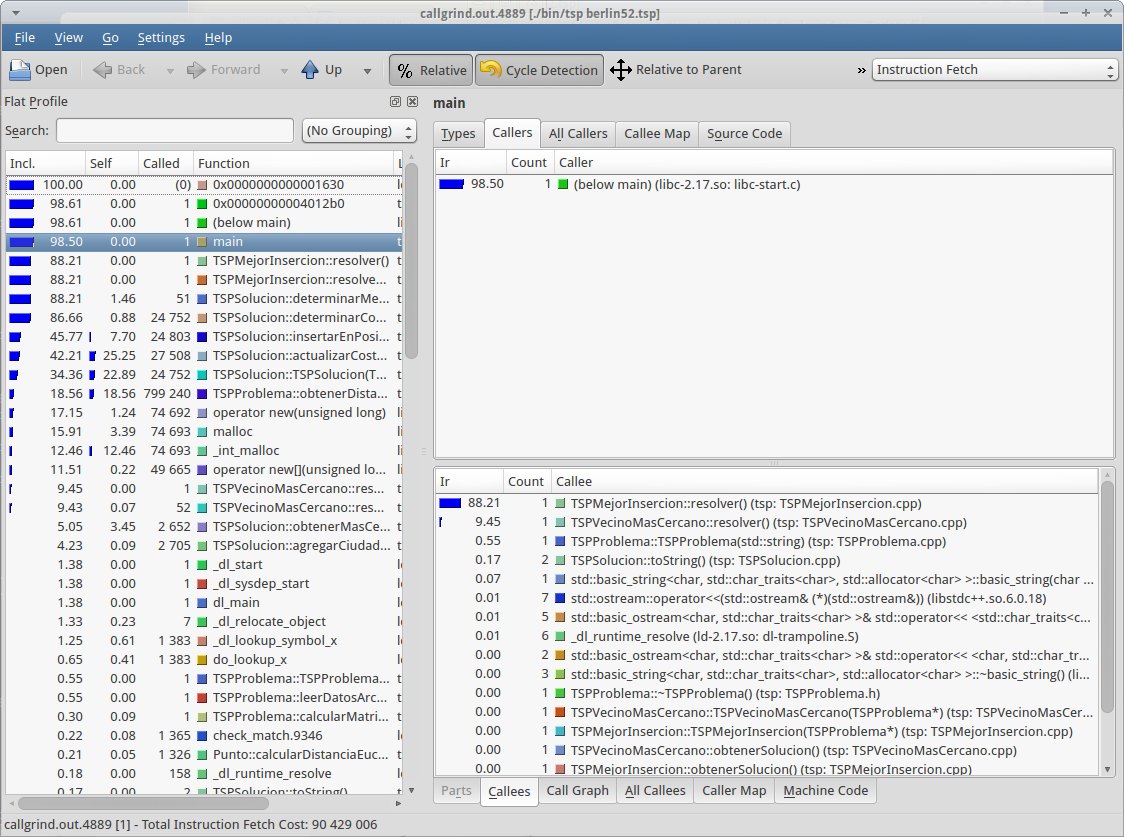
\includegraphics[scale=0.40]{kcachegrind1.png}
\end{center}

En la ventana de la izquierda aparece desglosada la lista general de llamadas
producidas junto con una estimación del tiempo total de ejecución usado por
cada método (función). Se aprecia que el método \textbf{resolver()} de la clase
\textbf{TSPMejorInsercion} ha consumido el $88\%$ del tiempo de ejecución. También
puede visualizarse un árbol con las llamadas realizadas:

\begin{center}
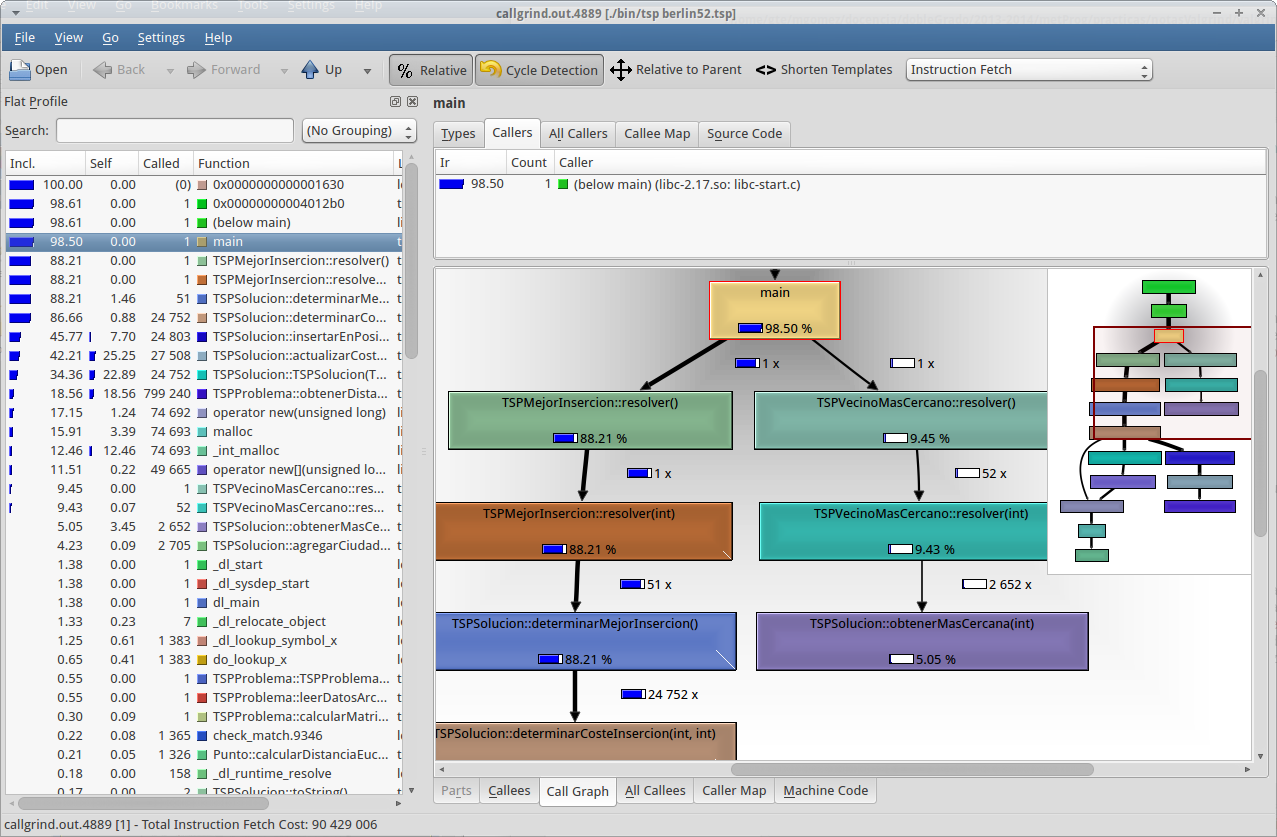
\includegraphics[scale=0.40]{kcachegrind2.png}
\end{center}

\end{document}
